\subsection{\texorpdfstring{\(\mathbf{A}_l\) 型系统 (\(l \geqslant 1\))}{A\_l 型系统 (l >= 1)}}

\begin{enumerate}
\def\labelenumi{(\Roman{enumi})}
\tightlist
\item
以及 (II) 设 \(V\) 是 \(E = R^{l + 1}\) 中方程为 \(\sum_{i=1}^{l + 1} \xi_i = 0\) 的超平面。将第 5 号中的 \(l\) 换成 \(l + 1\)，我们得到一个 \(R'\) 的 \(B_{l + 1}\) 型系统，它位于 \(E\) 中，其基为
\end{enumerate}

\[
\alpha_ {1} = \varepsilon_ {1} - \varepsilon_ {2}, \alpha_ {2} = \varepsilon_ {2} - \varepsilon_ {3}, \dots , \alpha_ {l} = \varepsilon_ {l} - \varepsilon_ {l + 1}. \alpha_ {l + 1} = \varepsilon_ {l + 1}.
\]

由于 \(\alpha_{1},\ldots,\alpha_{l}\) 生成 V，\(R=R^{\prime}\cap V\) 是 V 中以 \((\alpha_{1},\ldots,\alpha_{l})\) 为基的根系（§ 1，第 7 号，命题 20 的推论 4）。根据第 5 号中的标量积计算，立即可知 R 是 \(A_{l}\) 型的。R 的元素是 \(\varepsilon_{i}-\varepsilon_{j}\)（\(i\neq j,1\leqslant i\leqslant l+1,1\leqslant j\leqslant l+1\)）。根的数目为 \(n=l(l+1)\)。正根是 \(\varepsilon_{i}-\varepsilon_{j}\)，其中 \(i<j\)。

\begin{enumerate}
\def\labelenumi{(\Roman{enumi})}
\setcounter{enumi}{2}
\item
  我们有 \(h = n / l = l + 1\)。
\item
  令 \(\tilde{\alpha} = \varepsilon_1 - \varepsilon_{l+1} = \alpha_1 + \alpha_2 + \cdots + \alpha_l\)，这是一个根。相对于 \((\alpha_i)\)，它的坐标之和为 \(l = h - 1\)。因此，\(\tilde{\alpha}\) 是最高根。
\end{enumerate}

当 \(l = 1\) 时，\(\tilde{\alpha} = \alpha_{1}\)，所以 \((\tilde{\alpha}|\alpha_{1}) = 2\)；群 \(W_{a}(R)\) 的 Coxeter 图为

当 \(l \geqslant 2\) 时，\((\tilde{\alpha}|\alpha_i) = 0\) 对 \(0 < i < l\) 成立，且 \((\tilde{\alpha}|\alpha_1) = (\tilde{\alpha}|\alpha_l) = 1\)。因此，扩展 Dynkin 图为：

\pandocbounded{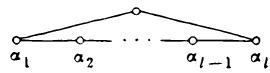
\includegraphics[keepaspectratio]{images/part002_36cfe44b.jpg}}

\begin{enumerate}
\def\labelenumi{(\Alph{enumi})}
\setcounter{enumi}{21}
\tightlist
\item
利用标量积将 V 与其对偶识别，我们有 \(\alpha^{\prime} = \frac{2\alpha}{(\alpha|\alpha)} = \alpha\) 对所有 \(\alpha \in R\) 成立，所以 \(R^{\prime} = R\)。
\end{enumerate}

对于形式 \(\Phi_{\mathbb{R}}\)，根的长度为 \(h^{-1/2} = (l + 1)^{-1/2}\)（§ 1，第 12 号）；因此 \(\Phi_{\mathrm{R}}(x,y) = (x|y)/2(l+1)\)。

我们有 \(\gamma (\mathbb{R}) = (l + 1)^2\)（§ 1，第 12 号，公式 (20)）。

\begin{enumerate}
\def\labelenumi{(\Roman{enumi})}
\setcounter{enumi}{5}
\tightlist
\item
  令 \((\omega_{i})_{1\leqslant i\leqslant l}\) 为基本权族。置
\end{enumerate}

\[
\omega_ {i} = \sum_ {j = 1} ^ {l + 1} \xi_ {i j} \varepsilon_ {j}. \quad \text { with } \xi_ {i j} \in \mathbf {R}.
\]

条件 \((\omega_{i}|\alpha_{j}) = \delta_{ij}\) 和 \(\omega_{i}\in V\) 给出

\[
\xi_ {i i} - \xi_ {i, i + 1} = 1, \quad \xi_ {i j} - \xi_ {i, j + 1} = 0 \text {   for   } j \neq i, \quad \sum_ {j = 1} ^ {l + 1} \xi_ {i j} = 0,
\]

由此容易得到

\[
\begin{array}{r l} \omega_ {i} & = \varepsilon_ {1} + \dots + \varepsilon_ {i} - \frac {i}{l + 1} (\varepsilon_ {1} + \dots + \varepsilon_ {l + 1}) \\ & = \frac {1}{l + 1} ((l - i + 1) (\alpha_ {1} + 2 \alpha_ {2} + \dots + (i - 1) \alpha_ {i - 1}) \\ & \quad + i ((l - i + 1) \alpha_ {i} + (l - i) \alpha_ {i + 1} + \dots + \alpha_ {l})). \end{array}
\]

\begin{enumerate}
\def\labelenumi{(\Roman{enumi})}
\setcounter{enumi}{6}
\tightlist
\item
  正根之和为
\end{enumerate}

\[
\begin{array}{r l} 2 \rho & = l \varepsilon_ {1} + (l - 2) \varepsilon_ {2} + (l - 4) \varepsilon_ {3} + \dots - (l - 2) \varepsilon_ {l} - l \varepsilon_ {l + 1} \\ & = l \alpha_ {1} + 2 (l - 1) \alpha_ {2} + \dots + i (l - i + 1) \alpha_ {i} + \dots + l \alpha_ {l}. \end{array}
\]

\begin{enumerate}
\def\labelenumi{(\Roman{enumi})}
\setcounter{enumi}{7}
\tightlist
\item
  在 \(\mathbf{E} = \mathbf{R}^{l + 1}\) 中引入第 4 号的子群 \(\mathrm{L}_0\)。设 \(p\) 是 E 到 V 的正交投影。由 § 1，第 10 号，命题 28，有
\end{enumerate}

\[
\mathrm{Q} (\mathrm{R}) = \mathrm{Q} \left(\mathrm{R} ^ {\prime}\right) \cap \mathrm{V} \neq \mathrm{L} _ {0} \cap \mathrm{V}, \text { and } \mathrm{P} (\mathrm{R}) = p \left(\mathrm{P} \left(\mathrm{R} ^ {\prime}\right)\right);
\]

由于 \(R'\) 的最后一个基本权与 V 正交，我们有 \(\mathrm{P}(\mathrm{R}) = p(\mathrm{Q}(\mathrm{R}')) = p(\mathrm{L}_0)\)。因此，\(\mathrm{P}(\mathrm{R})\) 是由 \(\varepsilon_i - \varepsilon_j\) 以及 \(p(\varepsilon_1) = \varepsilon_1 \to (l + 1)^{-1} \sum_{i=1}^{l+1} \varepsilon_i\) 生成的群，所以

\[
\mathrm{P} (\mathrm{R}) = \mathrm{Q} (\mathrm{R}) + \mathbf {Z} \left(\varepsilon_ {1} - (l + 1) ^ {- 1} \sum_ {i = 1} ^ {l + 1} \varepsilon_ {i}\right).
\]

现在，\(l + 1\) 是满足 \(m > 0\) 且 \(mp(\varepsilon_1) \in Q(R)\) 的最小整数。因此，\(P(R)/Q(R)\) 同构于 \(\mathbf{Z}/(l + 1)\mathbf{Z}\)，连接指标为 \(l + 1\)。

\begin{enumerate}
\def\labelenumi{(\Roman{enumi})}
\setcounter{enumi}{8}
\tightlist
\item
  以及 (X) 对 V 的任意自同构 g，令 \(\varphi(g)\) 为将 g 延拓到 E 且保持 \(\varepsilon_{1} + \varepsilon_{2} + \cdots + \varepsilon_{l}\) 不变的自同构。若 g 是正交反射 \(s_{\varepsilon_{i} - \varepsilon_{j}}|V\)，则 \(\varphi(g)\) 等于 \(s_{\varepsilon_{i} - \varepsilon_{j}}\)；后者将 \(\varepsilon_{i}\) 与 \(\varepsilon_{j}\) 互换，并保持所有下标 k 与 i、j 不同的 \(\varepsilon_{k}\) 不变。令
\end{enumerate}

\[
X = \left\{\varepsilon_ {1}, \varepsilon_ {2}, \dots , \varepsilon_ {l + 1} \right\}.
\]

于是，\(g \mapsto \varphi(g)|_{\mathbf{X}}\) 是从 \(W(\mathbf{R})\) 到 \(\mathbf{X}\) 的对称群的同构。因此，\(W(\mathbf{R})\) 同构于对称群 \(\mathfrak{S}_{l+1}\)，其阶为 \((l+1)!\)。

对称代数 \(\mathbf{S}(\mathrm{E})\) 可与 E 上的多项式函数代数 \(\mathrm{P}(\xi_1, \xi_2, \ldots, \xi_{l+1})\) 作规范识别。令 \(\mathrm{G} = \varphi(\mathrm{W}(\mathrm{R}))\)。由上一段，\(\mathbf{S}(\mathrm{E})^{\mathrm{G}}\) 中在 G 下不变的 \(\mathbf{S}(\mathrm{E})\) 元素所成的集合就是对称多项式的集合（《代数》，第 V 章，附录 I），因而（同上）是由下列函数生成的代数

\[
s _ {i} ^ {\prime} = \sum_ {\tau \in \mathfrak {S} _ {l + 1}} \xi_ {\tau (1)} \xi_ {\tau (2)} \dots \xi_ {\tau (i)} \quad (1 \leqslant i \leqslant l + 1).
\]

代数 \(\mathbf{S}(\mathrm{V})\) 可识别为多项式函数在 \(\mathrm{V}\) 上的限制所成的代数，这些多项式函数定义在 \(\mathrm{E}\) 上。若 \(\mathrm{P} \in \mathbf{S}(\mathrm{E})^{\mathrm{G}}\)，则 \(\mathrm{P}\) 在 \(\mathrm{V}\) 上的限制显然在 \(\mathrm{W}(\mathrm{R})\) 下不变。反之，若 \(\mathrm{Q} \in \mathbf{S}(\mathrm{V})^{\mathrm{W}(\mathrm{R})}\)，则存在 \(\mathrm{P} \in \mathbf{S}(\mathrm{E})\) 延拓 \(\mathrm{Q}\)；将 \(\mathrm{P}\) 替换为 \(((l + 1)!)^{-1} \sum_{g \in \mathrm{G}} g(\mathrm{P})\)，所得多项式的限制与 \(\mathrm{P}\) 在 \(\mathrm{V}\) 上的限制相同。我们可以设 \(\mathrm{P} \in \mathbf{S}(\mathrm{E})^{\mathrm{G}}\)。因此，\(\mathbf{S}(\mathrm{V})^{\mathrm{W}(\mathrm{R})}\) 由 \(s_i = s_i'|\mathrm{V}\) 生成。现在 \(s_1 = 0\)。此外，在 \(\mathbf{R}\) 上，\(\mathbf{S}(\mathrm{V})^{\mathrm{W}(\mathrm{R})}\) 的分式域的超越次数为 \(l\)，所以 \(s_i\)（\(2 \leqslant i \leqslant l + 1\)）代数独立。由于 \(s_i\) 的次数为 \(2, 3, \ldots, l + 1\)，\(\mathrm{W}(\mathrm{R})\) 的指数为

\[
1, 2, 3, \dots , l.
\]

\begin{enumerate}
\def\labelenumi{(\Roman{enumi})}
\setcounter{enumi}{10}
\tightlist
\item
  当 \(l = 1\) 时，A(R) = W(R) = Z/2Z 且 \(w_0 = -1\)。
\end{enumerate}

当 \(l \geqslant 2\) 时，令 \(\varepsilon \in A(R)\) 为把 \(\alpha_i\) 变为 \(\alpha_{l+1-i}\) 的自同构。显然，由 \(\varepsilon\) 诱导的自同构是 Dynkin 图的唯一非平凡自同构。群 \(A(R)/W(R)\) 同构于 \(Z/2Z\)。由 (IX) 和 (X)，-1 是属于 \(A(R)\) 但不属于 \(W(R)\) 的元素，因此 \(A(R)\) 同构于 \(W(R) \times Z/2Z\)。我们有 \(w_0 = -\varepsilon\)。

\begin{enumerate}
\def\labelenumi{(\Roman{enumi})}
\setcounter{enumi}{11}
\tightlist
\item
  群 \(\mathrm{P}(\mathrm{R}^{-})/\mathrm{Q}(\mathrm{R}^{-})\) 是阶为 \(l+1\) 的循环群，并通过循环置换作用于扩充的 Dynkin 图。若 \(l\geqslant2\)，\(\mathrm{A}(\mathrm{R})/\mathrm{W}(\mathrm{R})\) 的唯一非恒等元素在 \(\mathrm{P}(\mathrm{R}^{-})/\mathrm{Q}(\mathrm{R}^{-})\) 上的作用是自同构 \(x\mapsto-x\)。
\end{enumerate}

